\documentclass[11.5pt, twoside, a4paper]{article}
\usepackage{graphicx, amssymb, amsmath, amsthm, xfrac, mathabx, upgreek, fancyhdr, float, underscore, url}
\usepackage[section]{placeins}

\begin{document}

\title{Intelligent Adaptive Systems: Assignment}
\author{Chanelle Lee}
\date{\today}
\maketitle

\section{Introduction}

\subsection{Adaptive Neuro-Fuzzy Inference System (ANFIS)} %Needs a bit more work
ANFIS is a `fuzzy inference system implemented in the framework of adaptive networks' developed in the early 1990s \cite{JangANFIS}. It is called a hybrid neuro-fuzzy technique as it uses the learning capabilities of neural networks to `tune' the membership functions of a Sugeno-type Fuzzy Inference Sytem. A limitation of ANFIS is that it uses supervised learning and as such needs training input-output data, which can be difficult to source for problems and for this task in particular the density of the training data can be a problem. In addition, as ANFIS tunes the membership functions to the training data, sometimes the training data can be learnt so well that 

\subsection{The Task}
The task of this assignment is to use ANFIS to derive a representation of the inverse kinematics of the Lynxmotion robotic arm. In order to investigate this, Matlab's anfis toolbox will be used, with the main questions to be explored:
\begin{enumerate}
\item What is the ideal density of training data? A balance between efficiency and effectiveness is needed; as the more training data points the more accurate the results, but the longer the system takes.
\item How to generate the initial fuzzy inference system; should genfis1 or genfis2 be used? 
\item For how many epochs should ANFIS run?
\item What should be the spread of the training data? Should the training data points be uniform over the workspace or concentrated near singularities?
\end{enumerate}

 Due to time constraints, the simpler problem of a two link arm will be used to investigate the first three questions; as the data sets required to train the system are much smaller, and so more exploration of parameter settings of the ANFIS is achievable. Then, the best parameters found will be used to train for a three link arm and as the three link arm gives a planar representation of the Lynxmotion arm, the final question will be investigated. Finally, these findings will be implemented on the Lynxmotion arm and compared against analytical solutions.

\section{Two Link Arm} %should this be link or joint?

For this section, the Lynxmotion arm will be reduced the to the two link problem as described in Fig.\ref{fig:2Link}\footnote{Alterred to match findings in Section\ref{sec:elbowIssues}}. 

\begin{figure} %Might be a bit large
\begin{center}
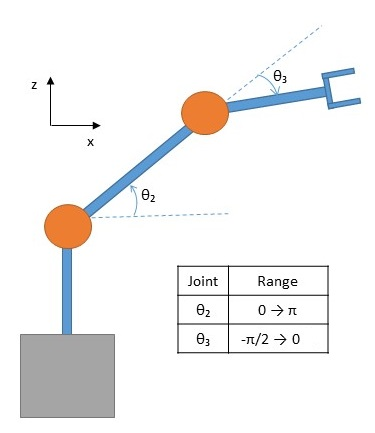
\includegraphics{2Link.jpg}
\caption{Two Link Robotic Arm \label{fig:2Link}}
\end{center}
\end{figure}

\subsection{Joint Angle Range Issues} \label{sec:elbowIssues}

When the experiements were first run there were very large errors in the cartesian and joint space (Table.\ref{tab:range})\footnote{Genfis1 with two membership functions, 100 data points and 500 epochs.} and this was discovered to be because the range $\theta_3$ was set to $\left[-\pi/2,\pi/2\right]$ meaning that for each point in cartesian space there could be two solutions in the joint space with either a positive or negative value for $\theta_3$. This corresponded to the fact that each point in cartesian space can be reached by the end effector in one of two configurations; elbow up or elbow down. This was solved by limiting the range of $\theta_3$ to only negative values, i.e. limiting the robotic arm to only elbow down configurations, which is much more realistic in terms of the Lynxmotion arms capabilities.

\begin{table}
\scalebox{0.7}{
\begin{tabular}{|c||c|c|c|c|c|c|c|}\hline
$\theta_3$ range & trnRMSE2 & chkRMSE2 & trnRMSE3 & chkRMSE3 & cartRMSE & cartMin & cartMax\\ \hline\hline
$\left[-\pi/2, \pi/2\right]$ & 0.3792 &  0.3794 &   0.7387  &  0.7389 &  35.7034  &  0.0497 &  99.4345\\ \hline
$\left[-\pi/2, 0\right]$ & 0.0312 &   0.0311  &  0.0682 &   0.0687  &  5.5590  &  0.0651  & 111.7742 \\ \hline
\end{tabular}}
\caption{Results from changing range of $\theta_3$. \label{tab:range}}
\end{table}


\subsection{Number of Epochs}
The number of epochs controls the length of time ANFIS spends tuning the membership functions of the Fuzzy Inference System (FIS) and setting this is a matter of comparing the accuracy attained against the time taken. In Fig.\ref{fig:2000Epochs}\footnote{Genfis1 with two membership functions and 100 data points} it is clear that if only the first fifty epochs are considered the training and validation errors of the joint angles are still falling and there is little evidence to show how far they might further fall, but when one thousand epochs are run there is clearly little improvement after five hundred epochs. Table.\ref{tab:epochs} also shows that the Root-Mean-Squared-Error (RMSE) in the cartesian space reduces by less than a tenth of a millimetre from five hundred to one thousand epochs despite it taking twice as long to run. Interestingly, there is also little change in the cartesian RMSE between one hundred epochs and five hundred epochs.. In conclusion, the best number of epochs to use for further experiments is five hundred as confidence can be had that training and validation errors in the joint angles have stabilised by this epoch, but there is little point continuing as neither the error in the joint angles or the cartesian RMSE appear to decrease enough to be beneficial.

\begin{figure}
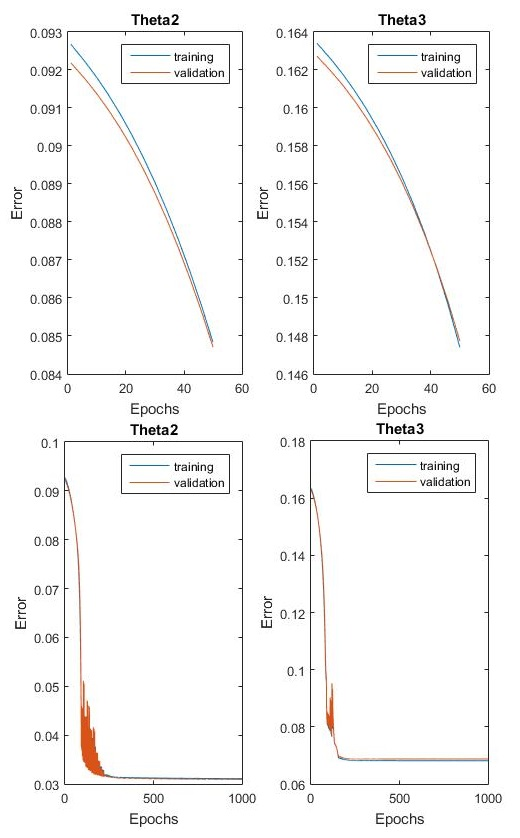
\includegraphics[width=\linewidth]{Epochs.jpg}
\caption{Two Link Arm with run for 50 and 1000 Epochs\label{fig:2000Epochs}}
\end{figure}

\begin{table} 
\scalebox{0.7}{
\begin{tabular}{|c | c | c | c | c | c | c | c | c | c  | c | } 
\hline
dataPoints & Epochs & MFs & trnRMSE2 & chkRMSE2 & trnRMSE3 & chkRMSE3 & cartRMSE & cartMin & cartMax & time \\ \hline \hline
100 &	50   &	2 &	0.0848 &	0.0847 &	0.1474 &	0.1477 &	8.9448 &	0.0728 &	63.0842  &	2.38 \\ \hline
100 &	100  &	2 &	0.0358 &	0.0356 &	0.0795 &	0.0801 &	5.8968 &	0.0425 &	25.2959  &	4.38 \\ \hline
100 &	500  &	2 &	0.0312 &	0.0311 &	0.0682 &	0.0687 &	5.5590 &	0.0651 &	111.7742 &	20.17 \\ \hline
100 &	1000 &	2 &	0.0311 &	0.0309 &	0.0681 &	0.0687 &	5.5723 &	0.0184 &	111.7176 &	39.92 \\ \hline
\end{tabular}}
\caption{Number of Epochs Experiment \label{tab:epochs}}
\end{table}

\subsection{Optimising Genfis1}
To investigate the best parameters using Genfis1 to create the FIS two loops were used to explore:
\begin{itemize}
\item The number of membership functions between two and ten.
\item The number of data points from ten, twenty, fifty, one hundred, two hundred and five hundred.
\end{itemize}

\subsubsection{Number of Membership Functions}
The number of membership functions is used by genfis1 to set the number of membership functions of each variable in the FIS \cite{genfis1} and this is important to explore as more membership functions can lead to an increase in accuracy. However, as an increase in membership functions also leads to an increase in hidden neurons in the neural network, too many can lead to overfitting of data, where the FIS has been trained to very good on the training data, but can diverge wildly in between. 

\subsubsection{Density of Training Data}

\subsection{Optimising Genfis2}
Genfis2 uses subtractive clustering to generate a Sugeno-type FIS structure \cite{genfis2} and in this experiment a genetic algorithm is used to try and determine optimal radii inputs for each joint. A genetic algorithm was chosen here, over any other type of optimisation algorithm, as it was feared that there would be many local optima, e.g. the optimal radius for each cluster. The fitness function used to evaluate the performance of the chromosomes is the cartesian RMSE mitigated slightly by time taken.

Time problems were experienced using the genetic algorithm, as the time taken for each generation is the length of time for fitness function (in this case genfis2 and anfis) to run multiplied by the population size. In terms of computational practicality, the length of time of the fitness function should in future be taken into account when considering the use of a genetic algorithm. 

\section{Three Link Arm}

Need to have another constraint to balance the new variable, using the pitch.

\section{Lynxmotion Arm}


\section{Appendix 1 - Experiment Result Tables Overflow}




\bibliographystyle{unsrt}
\bibliography{IAS}{}


\end{document}